\chapter{Review of Related Literature}
\label{sec:rrl} 

\section{dPCR Droplet Classification Methods}
\label{sec:dpcrclassifiers}

\subsection{Droplet dPCR (ddPCR) System}
\label{sec:ddpcrsystem}
The most common method in classifying positive and negative droplets is by enforcing a hard threshold. Generally, all droplets with a fluorescence amplitude greater than this threshold are then classified as positive, and negative otherwise. 

One popular tool incorporated with automatic thresholding is the QuantaSoft software. The QuantaSoft software is the dPCR analysis tool that comes with the Bio-Rad droplet dPCR (ddPCR) System package. It allows for the setting up of sample and experiments, running and controlling the instrument, and finally, the analysis of the NA concentration \cite{Bio-Rad2019}. According to the Bio-Rad Laboratories website (https://www.bio-rad.com), it has been a leading product developer for 65 years in the research fields of life science and clinical diagnostics. Among its popular focus areas, dPCR is one of its most featured technology, providing ddPCR instruments; kits, reagents and assays; and other consumables. Several studies in hospitals \cite{Lopez2016,Chen2018,Abed2017,Tagliapietra2020}, public health \cite{Hussain2017,Nystrand2018}, food safety \cite{Chen2020,Capobianco2020,Basanisi2020}, upto environmental quality \cite{Hamaguchi2018,Jahne2020,Dobnik2016,Mauvisseau2019} have found the Bio-Rad QuantaSoft dPCR systems useful for their analyses. 

Of all the QuantaSoft software features, the focus of this section is on its threshold setting. By default, QuantaSoft sets an automatic threshold to the single-well or multiple-well amplitude data; a demonstration is shown in \figref{fig:demoQuantThreshold}. As with other automated tools, its documentation recommends reviewing this threshold to make changes if needed; and thus, manually setting the threshold is also allowed. Unfortunately, the calculation of the automatic threshold is not publicly available.

\begin{figure}[h]
    \centering
    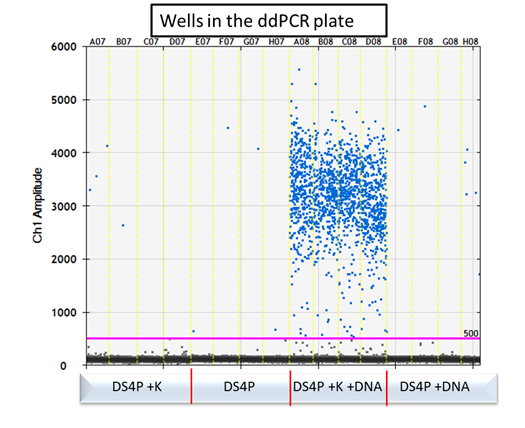
\includegraphics[max size={\textwidth}{\textheight}]{quantasoftThreshold.png}
    \caption[QuantaSoft threshold from a study]{QuantaSoft threshold in pink line from \cite{hussainThreshold}}
        \label{fig:demoQuantThreshold}
\end{figure}

The evaluation of the QuantaSoft software show exemplary results from the food safety study of \citeA{Basanisi2020}, whereby nine pure meat samples were discriminated with 100\% diagnostic accuracy, sensitivity, and specificity. However, upon checking the authenticity of twenty commercially available meat products, twelve samples were said to contain DNA traces of other animals not declared. Among the several reasons for this high detection, \citeA{Basanisi2020} suggests the need for a highly sensitive and specific test in the molecular level. Observation of NA molecules can be done through their droplet fluorescence in a dPCR assay.

Assessing the QuantaSoft software's ability to classify droplets, it was shown that for samples exhibiting a substantial amount of intermediate fluorescence, the system fails to determine a threshold (outputs "No call"). This was the case in the two bacteria study of \cite{Dreo2014}, that were ran on very high concentrations. In the case of low bacteria concentrations, droplets near the negative droplets were classified as positives. This study concluded that the QuantaSoft software requires a well-optimized assay with good discrimination of positive and negative droplets for its threshold to be reliable.


\subsection{Manual Global Threshold (MTg)}
\label{sec:manthreshold}
As opposed to the automatic threshold, \citeA{Dreo2014} proposes setting a manual global threshold (MTg) determined by no template control (NTC) samples. This takes into consideration that individual assays behave differently, and could require expert intervention. For example, the threshold for a well-optimised assay was defined as the NTC mean + 6 standard deviations; on the other hand, a noisy assay had its threshold set above the highest value in NTC samples. It is expected in the latter example that the sensitivity would be lower, due to its high threshold. However, the paper claims that this resulted in high analytical sensitivity for that assay. A major disadvantage in this approach is the clear definition or guidelines in setting the MTg; this consequently will cause reproducibility issues for succeeding experiments and external researchers.

\subsection{Kernel Density Estimation (KDE)}
\label{sec:peakdetectionkde}
The positive and negative droplet classification can be framed as a clustering problem. One solution is by using the popular theory of kernel density estimation (KDE); whereby each data point influence is modeled using a kernel function — frequently Gaussian distributed, and the sum of all the kernel functions would be the overall density of the data. Clusters can then be derived from the estimated densities depending on its application \cite{Hinneburg2003}.

KDE has been particularly helpful in spatial analysis. Clusters were detected in areas with diabetes in Berlin \cite{Kauhl2016}, HCV hepatitis C virus in Massachusetts \cite{Stopka2017}, and crime hotspots in Brazil \cite{Junior2019}. For other data types, KDE clustering has been improved in an algorithm developed by \shortciteA{Rodriguez2014}, called clustering by fast search and find of density peaks. This technique has piqued the interests of many researchers; thereby further improving the original limitations via DNA genetic algorithm \cite{Zang2017}, heat diffusion \cite{Mehmood2016}, and entropy of data field \cite{Wang2016}.  

Although not named in the dPCR optimization paper of \citeA{Lievens2016}, cloudy is the name of the function in their supplementary source code file that calculates the threshold from the clusters found by using Gaussian KDE. The following steps explain this in more detail:
\begin{enumerate}
    \item Estimate the density function of the fluorescence using a Guassian kernel density with a minimum bandwith of 50
    \item Identify density peaks using a sliding window approach. The subsequent steps will differ according to if one, two, or more than three peaks were found.  But generally, the proceeding steps are followed.
    \item For each population found through the peaks, its location and spread is initially estimated using the median \(\hat{\mu}\) and \(\hat{\sigma}\). Assuming normality, the latter is estimated as half the peak width at 60-65\% of its maximum height.
    \item Refine the estimates using a reiterative method, first initialized with \(a=4\).
    \item Re-estimate \(\hat{\mu}\) and \(\hat{\sigma}\) using only the observations within \(\hat{\mu} \pm (a \cdot \hat{\sigma})\).
    \item Recalculate \(a=4.55 + 0.35 \cdot log(k) + 0.045 \cdot log(k)^2\); where \(k\) is the kurtosis of the distribution
    \item Repeat steps 5-6 until stabilization.
    \item After stabilizing the estimates for all the population, the last step is different when either including or excluding rain in the final categorization. 
    \begin{enumerate}
        \item If rain is included as a category, observations within \(\hat{\mu} \pm (a \cdot \hat{\sigma})\) are then classified as members of that population; observations not falling within any population are classified as rain.
        \item If rain categorization is not of interest, then a threshold \(\theta=\hat{\mu_n} + 1.5 \cdot a_n + \hat{\sigma_n}\) is calculated; where \(n\) is a population.  
    \end{enumerate}

\end{enumerate}

In summary, the cloudy algorithm uses the Gaussian kernel density and normality assumptions to detect peaks, which are then considered as populations. From then population density parameters are estimated based on specified formulas. A range or a single threshold is then calculated for classifying droplets as positive, negative, or optionally, rain.

Special cases such as overlapping population boundaries and threshold placement problems are also checked in their source code. It is worth noting that in step 6, the formula for re-calculating \(a\) for density parameter estimation is based on the analysis of their in-house data, and should be used with caution when implementing for other unobserved NA targets. The rain classification rule in step 8(a) also poses a problem for fluorescence densities that are heavily skewed. \figref{fig:skeweddist} left panel reveals the distribution of negative droplets to be heavily skewed to the right, thereby causing their exclusion to be labeled as negative due to the symmetry of the categorization rule (right panel).

\begin{figure}[h]
    \centering
    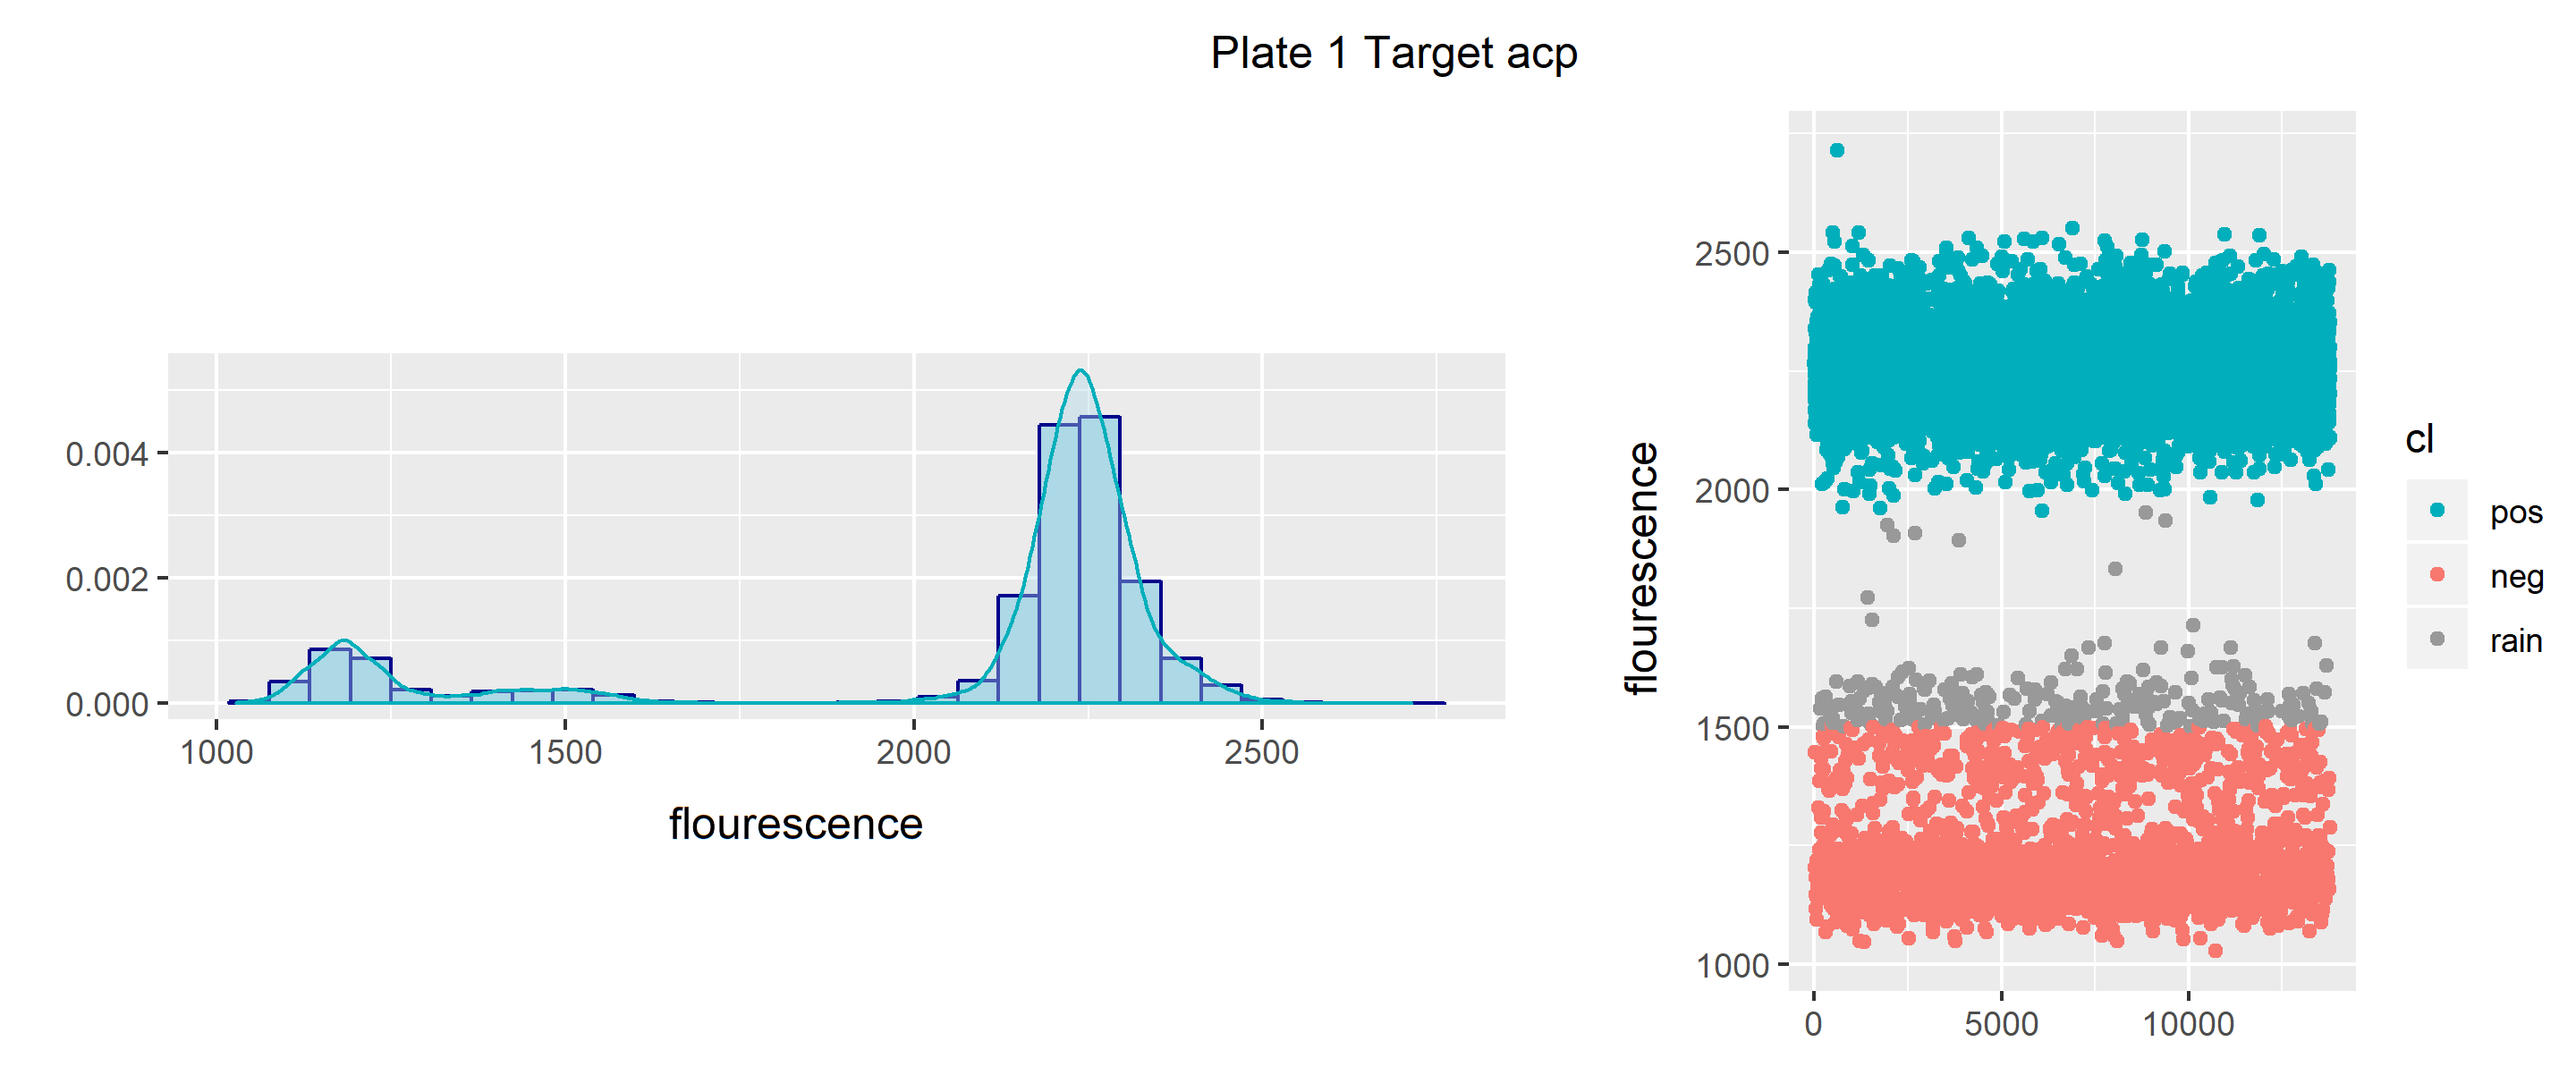
\includegraphics[max size={\textwidth}{\textheight}]{skeweddist.png}
    \caption[Fluorescence distribution of DNA target acp]{One replicate of the DNA target acp Plate 1 from \citeA{Lievens2016} dataset. Left panel shows the fluorescence densities. Right panel is the result of droplet categorization using cloudy}
        \label{fig:skeweddist}
\end{figure}

It is noted that the context of the threshold setting here is based on in-house data for studying dPCR experiment optimization, and not necessarily as a classifier for external data. The constant threshold criterium enables the control for other PCR experimental factors, such as sonication, PCR enhancers, annealing conditions, and number of cycles, to achieve optimization or diminishing rain droplets for dPCR experiments.

\subsection{K-Nearest-Neighbors (KNN)}
\label{sec:knn}
Based on the research papers curated by \citeA{Peterson:2009}, K-nearest-neighbor (KNN) is a unsupervised clustering approach that should be among the first methods considered for data with little to no information about its distribution. This clustering method operates on the chosen distance measure — commonly the Euclidean distance — between the observations. Due to its simplicity, data from various fields have applied KNN such as in a movie recommendation system \cite{Ahuja2019}, climate classification \cite{Shi2020}, breast cancer diagnostics \cite{Mittal2019}, among others.

An open-source tool developed by \shortciteA{Jones2014}, called definetherain, utilizes the KNN algorithm in identifying rain droplets. According to their research, they claim that definetherain is accurate in estimating assays with low template numbers, which is particularly applicable in research fields such as the HIV-1 cure research. definetherain follows these steps for classification:
\begin{enumerate}
    \item Setup a positive control sample of known input copy numbers. 
    \item Cluster the droplets using kNN with \(k=2\). The cluster on the left is the negative cluster, and on the right is the positive cluster. 
    \item Observations between the range of the negative cluster's mean + 3 standard deviations and the positive cluster's mean - 3 standard deviations are classified as rain.
    \item Rain droplets are not included in the final calculation of the concentration estimate.
\end{enumerate}

\begin{figure}[h]
    \centering
    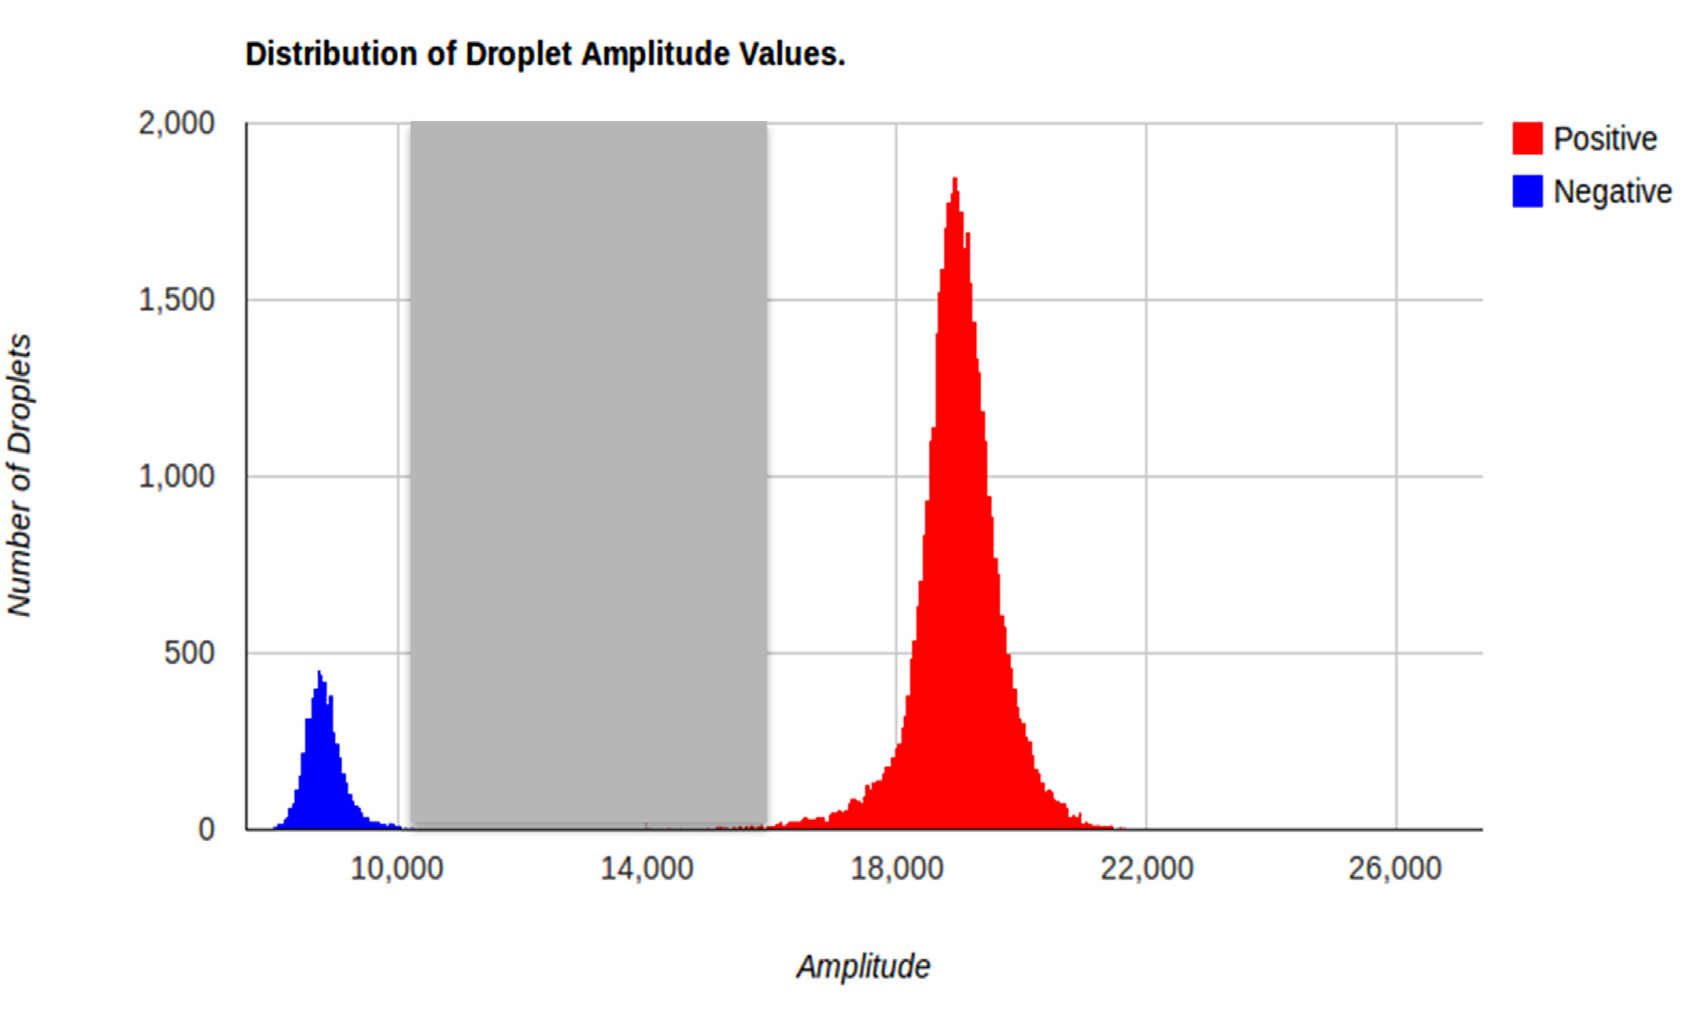
\includegraphics[max size={\textwidth}{\textheight}]{dtrsample.png}
    \caption[Determined thresholds calculated by definetherain]{Determined thresholds calculated by definetherain, reprinted from \cite{jonesThreshold}}
        \label{fig:dtrsample}
\end{figure}

Unlike the other methods discussed here, this tool produces two cutoff values — one for each cluster. The droplets falling between these two values are classified as rain. These cutoff values are solely dependent on the control sample. The disadvantage of this is that the control has to be representative of the NA target; otherwise, concentration estimates would be biased. 


% TODO - Studies that use dtr ? 


\subsection{Model-Based Clustering}
\label{sec:modelbasedclustering}
As opposed to the distance-based clustering in Section \ref{sec:knn}, a probabilistic approach is achieved with model-based clustering. According to \citeA{Mcnicholas2016}, in this approach, a cluster is defined as a unimodal component within a finite mixture model. The mixture model has to be appropriate in such that its parameters are flexible for fitting the characteristics of the data. Each observation, therefore, has a calculated probability of it belonging to a group. Using model-based clustering, studies have shown abstract data types with satisfactory outcomes. One example is image data in the study of \cite{Choy2017}. They were able to perform image segmentation using the generalized Gaussian density model. Each cluster formed is interpreted as an object, and the number of which is identified via a validation technique. Their algorithm was able to segment objects such as a starfish, cat, or tree in photographs. Additionally, using genetic data, \citeA{Li2018} discovered a potential differentially-variable microRNA (miRNA) not yet been reported in literature, upon fitting a three-component multivariate normal distribution to miRNA expression levels.


\shortciteA{Jacobs2017} developed Umbrella, a model-based clustering for dPCR droplets available in source code (https://github.com/statOmics/umbrella). After providing a representative NTC sample(s), the procedure follows a series of estimation and assumptions in deriving the final estimated concentration. An oversimplification of the Umbrella procedure, that skips the detailed steps for handling specific cases, are as follows:
\begin{enumerate}
    \item The NTC distribution \(f_0(x)\) is assumed to follow a unimodal distribution. The location and variation is estimated by the mode and mean of absolute deviation (MAD), respectively.
    \item The fluorescence intensitities \(x\) observed in partitions of a target partition set \(A\) is assumed to have a mixture density 
    \[f_A(x) = p_{0,A}f_{0,A}(x) + (1-p_{0,A})f_{1,A}(x)\]
    \begin{itemize}
        \item \(p_{0,A}\) = proportion of negative partitions
        \item \(f_{0,A}(x)\) = densities of the partitions without target copy (null component of the target partition set \(A\))
        \item \((1-p_{0,A})\) = proportion of positive partitions
        \item \(f_{1,A}(x)\) = densities of the partitions with target copy
    \end{itemize}
    \item Begin estimating the parameters by first aligning the modes of  the null component of \(f_A(x)\) and the NTC reference \(f_0(x)\).
    \item Discretize the aligned distributions by generating a histogram with the same bins.
    \item The bin counts of the aligned distribution are modeled using a Poisson regression model, resulting in estimates for \(\hat{p}_{0,A}\),\(\hat{f_{0}}(x)\), and \(\hat{f_{A}}(x)\).
    \item The posterior probability that partition \(i\) is void of the NA target with fluorescence intensity \(x_i\) of partition set \(A\), \(\hat{p_{0,A}}\), can be defined from the estimated \(\hat{p}_{0,A}\) from the previous step as
    \[ \hat{p}_{i,0,A}=\hat{p}_{0,A}\left(\begin{array}{c}\hat{f}_{0,A}(x_i)\\ \hat{f}_{A}(x_i)\end{array}\right) \]
    \item The Umbrella threshold estimator is then determined by the estimated \(\hat{p}_{i,0,A}\). For intensity value \(i\), the interpretation of the posterior probabilities are 
    \begin{itemize}
        \item \(\hat{p}_{i,0,A} > 80\%\) are considered negative partitions with a probability of \(\leq20\%\) to be false negatives
        \item \(\hat{p}_{i,0,A} < 5\%\) are considered positive partitions with a probability of \(\leq5\%\) to be false positives
        \item \(5\% \leq \hat{p}_{i,0,A} \leq 80\%\) are considered as rain
    \end{itemize}
\end{enumerate}


The mode and MAD, as the location and spread estimators for the null NTC distribution, \(f_{0}(x)\), are chosen due to its robustness and insensitivity to skewed tails. Only observations within 10 deviations of the mode are included for the null model.

Following the assumption of a mixture density in step 2, unlike most model-based clustering algorithms, Umbrella does not assume normal densities for \(f_{1,A}(x)\) and \(f_{0,A}(x)\), the partitions with and without the NA target, respectively. This is due to the exhibition of dPCR fluorescence intensities to be non-normal, as clusters tend to have heavy tails to the left or to the right. The solution for this is the use of non-parametric density estimation in step 3.

After estimating all the components in the mixture model from steps 3 - 5, the component of interest \(\hat{p_{0,A}}\) is then used to determine \(\hat{p}_{i,0,A}\) in step 6. Finally, this is used as the basis for Umbrella threshold estimator in step 7. It is cautioned that Umbrella may not be precise in detection experiments for low copy samples, as classifying individual samples is not the strength of this method.



\section{Expectation-Maximization (EM) Clustering}
\label{sec:emclustering}
% TODO - Expectation Maximization
